\documentclass[11pt]{article}
\usepackage{graphicx, fancyhdr}
\usepackage{amsmath, amsfonts}
\usepackage{color, hyperref}
\usepackage{enumerate}
\usepackage{longtable}
\providecommand{\tightlist}{%
  \setlength{\itemsep}{0pt}\setlength{\parskip}{0pt}}
 
\newcommand{\blue}[1]{{\color{blue} #1}}

\setlength{\topmargin}{-.375 in}
\setlength{\textheight}{8.75 in}
\setlength{\textwidth}{6.5 in}
\setlength{\evensidemargin}{0 in}
\setlength{\oddsidemargin}{0 in}
\setlength{\parindent}{0 in}
\renewcommand{\headrulewidth}{0.4pt}
\renewcommand{\footrulewidth}{0.4pt}

\lhead{Stat 305} 
\chead{Competency Quiz 4} 
\rhead{Tuesday, April 18}
\lfoot{Spring 2019}
\cfoot{\thepage} 
\rfoot{} 

\def\Exp#1#2{\ensuremath{#1\times 10^{#2}}}
\def\Case#1#2#3#4{\left\{ \begin{tabular}{cc} #1 & #2 \phantom
{\Big|} \\ #3 & #4 \phantom{\Big|} \end{tabular} \right.}

\begin{document}
\pagestyle{fancy} 

Show \textbf{all} of your work on this assignment and answer each question fully in the given context. You have 20 minutes. Each problem is designed to take 10 minutes. All answers in a topic must be correct for any credit for that topic. You may attempt multiple topics. You may use a calculator on this competency quiz. \\

\begin{enumerate}
\def\labelenumi{\arabic{enumi}.}
\item
  \textbf{Competency Topic: Discrete Random Variables}

  Suppose that \(X\) is a discrete random variable with the following
  probability function:
  \[f(x) = \begin{cases} \dfrac{x^2}{c} & x = -3, -2, -1, 0, 1, 2, 3 \\ 0 & o.w \end{cases}\]
  where \(c\) is a constant.

  \begin{enumerate}
  \def\labelenumii{\alph{enumii}.}
  \tightlist
  \item
    Find the value of \(c\) that makes \(f(x)\) a valid probability
    function. \vspace{4cm}
  \item
    Find \(P(X \ge 2)\). \vspace{4cm}
  \item
    Find \(E(X)\).
  \end{enumerate}
\end{enumerate}

\newpage

\begin{enumerate}
\def\labelenumi{\arabic{enumi}.}
\setcounter{enumi}{1}
\item
  \textbf{Competency Topic: Continuous Random Variables}

  The mean-0 Laplace distribution is continuous distribution with the
  following probability density function:
  \[f(x) = \dfrac{1}{2\alpha} \exp\left(-\dfrac{|x|}{\alpha}\right) \; -\infty < x < \infty\]
  where \(\alpha\) is a parameter which takes positive values (note:
  \(|x|\) is the absolute value of \(x\)).

  \begin{enumerate}
  \def\labelenumii{\alph{enumii}.}
  \tightlist
  \item
    Show that regardless of the value of \(\alpha\) the pdf above is
    symmetric (that is, show that \(f(-x) = f(x)\)). \vspace{3cm}
  \item
    Using the plot below, provide a rough sketch of the following pdfs:
  \end{enumerate}

  \begin{itemize}
  \item
    \begin{enumerate}
    \def\labelenumii{(\arabic{enumii})}
    \tightlist
    \item
      the pdf of a variable with \(\alpha = 0.5\).
    \end{enumerate}
  \item
    \begin{enumerate}
    \def\labelenumii{(\arabic{enumii})}
    \setcounter{enumii}{1}
    \tightlist
    \item
      the pdf of a variable with \(\alpha = 1\). (for the sketch, show
      the values of the pdfs when \(x = -2, -1, 0, 1, 2\))
    \end{enumerate}
  \end{itemize}
\end{enumerate}

\begin{center}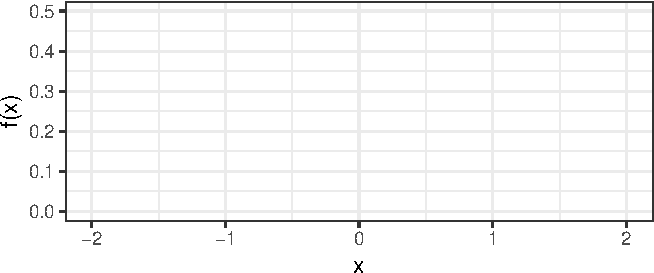
\includegraphics[width=.9\linewidth,height=.4\linewidth]{stat305-cq4_files/figure-latex/unnamed-chunk-2-1} \end{center}

\begin{enumerate}
\def\labelenumi{\alph{enumi}.}
\setcounter{enumi}{2}
\tightlist
\item
  Based on your sketch, would a random variable with \(\alpha = 0.5\)
  have a larger or smaller variance than a random variable with
  \(\alpha = 1\)?
\end{enumerate}

\newpage

\begin{enumerate}
\def\labelenumi{\arabic{enumi}.}
\setcounter{enumi}{2}
\item
  \textbf{Competency Topic: Joint Distributions}

  Suppose that \(X\) is a random variable with an exponential
  distribution with mean \(\lambda\). That is
  \[f_X(x) = \begin{cases} \dfrac{1}{\lambda} \exp\left(-\dfrac{x}{\lambda}\right) & x \ge 0 \\ 0 & otherwise \end{cases}\]
  and suppose that a random variable \(Y\) follows an exponential
  distribution that depends on the value taken by \(X\) so that
  \[f_Y|X(y|x) = \begin{cases} \frac{1}{x} & 0 \le y \le x \\ 0 & otherwise \end{cases}\]

  \begin{enumerate}
  \def\labelenumii{\alph{enumii}.}
  \tightlist
  \item
    Sketch the conditional probability density function of \(Y\) given
    that \(X = 4\).
  \end{enumerate}
\end{enumerate}

\begin{center}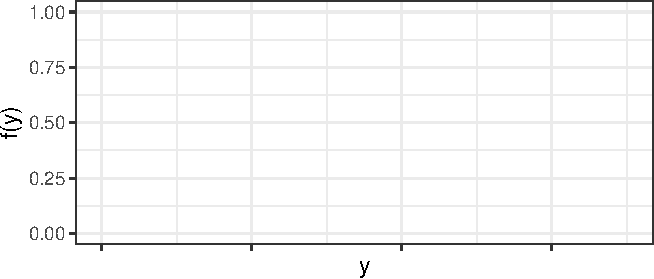
\includegraphics[width=.9\linewidth,height=.4\linewidth]{stat305-cq4_files/figure-latex/unnamed-chunk-3-1} \end{center}

\begin{enumerate}
\def\labelenumi{\alph{enumi}.}
\setcounter{enumi}{1}
\tightlist
\item
  Find the joint probability function, \(f_{XY}(x, y)\). \vspace{3cm}
\end{enumerate}

\newpage

\begin{enumerate}
\def\labelenumi{\arabic{enumi}.}
\setcounter{enumi}{3}
\item
  \textbf{Competency Topic: Functions of Random Variables}

  Suppose that \(W_1, W_2, ...\) are independent random variables each
  with the same expected value \(\mu\) and variance \(\sigma^2\). We
  define a random variable \(U_n\) as a linear combination of \(n\) of
  these random variables using:
  \[U_n = 2^{-1} W_1 + 2^{-2} W_2 + 2^{-3} W_3 + \ldots + 2^{-n} W_n\]
  note: if \(r \ge 1\), the
  \(r^{-1} + r^{-2} + \ldots r^{-n} = \sum_{k=1}^n r^{-k} = \dfrac{r^{n-1} - 1}{r^n - r^{n-1}}\)

  \begin{enumerate}
  \def\labelenumii{\alph{enumii}.}
  \tightlist
  \item
    Find an expression for \(E(U_n)\) (hint: it will contain \(\mu\) and
    \(n\)). \vspace{5cm}
  \item
    Find an expression for \(Var(U_n)\) (hint: it will contain
    \(\sigma^2\) and \(n\)).
  \end{enumerate}
\end{enumerate}

\end{document}
